\documentclass[a4paper,14pt]{article}

\usepackage{comment} % Para comentar várias linhas ao mesmo tempo

%matemática
\usepackage{amsmath}
\usepackage{amssymb}

%diagramação
\usepackage{extsizes}
\everymath{\displaystyle}
\usepackage{geometry}
\usepackage{fancyhdr}
\usepackage{multicol}
\usepackage{graphicx}
\usepackage[brazil]{babel}
\usepackage[shortlabels]{enumitem}
\usepackage{cancel}
\usepackage{textcomp}
\usepackage{tcolorbox}

%tabelas
\usepackage{array} % Para melhor formatação de tabelas
\usepackage{longtable}
\usepackage{booktabs}  % Para linhas horizontais mais bonitas
\usepackage{float}   % Para usar o modificador [H]
\usepackage{caption} % Para usar legendas em tabelas
\usepackage{wrapfig} % Para usar tabelas e figuras flutuantes
\usepackage{xcolor} % Para cores do fundo de tabelas
\usepackage{colortbl} % Para cores do fundo de tabelas

%tikzpicture
\begin{comment}
	\usepackage{tikz}
	\usepackage{scalerel}
	\usepackage{pict2e}
	\usepackage{tkz-euclide}
	\usetikzlibrary{calc}
	\usetikzlibrary{patterns,arrows.meta}
	\usetikzlibrary{shadows}
	\usetikzlibrary{external}
\end{comment}


%pgfplots
\usepackage{pgfplots}
\pgfplotsset{compat=newest}
\usepgfplotslibrary{statistics}
\usepgfplotslibrary{fillbetween}

%colours
\usepackage{xcolor}



\columnsep=2cm
\hoffset=0cm
\textwidth=8cm
\setlength{\columnseprule}{.1pt}
\setlength{\columnsep}{2cm}
\renewcommand{\headrulewidth}{0pt}
\geometry{top=1in, bottom=1in, left=0.7in, right=0.5in}

\pagestyle{fancy}
\fancyhf{}
\fancyfoot[C]{\thepage}

\begin{document}
	
	\noindent\textbf{8FMA111 - Matemática} 
	
	\begin{center}Revisão: equação de reta (Versão estudante)
	\end{center}
	
	\noindent\textbf{Nome:} \underline{\hspace{10cm}}
	\noindent\textbf{Data:} \underline{\hspace{4cm}}
	
	%\section*{Questões de Matemática}
	
	\begin{multicols}{2}
		\noindent \begin{itemize} \item Toda equação da forma $Ax + By + C = 0$, onde $A \neq 0$ ou $B \neq 0$, tem como gráfico uma reta no plano cartesiano e vice-versa. 
		\item Toda reta que não é paralela ao eixo $Oy$ admite uma equação reduzida da forma $y = ax + b$, em que $a$ é o coeficiente angular da reta (tangente do ângulo de inclinação) e $b$ é o coeficiente linear da reta (ordenada do ponto de intersecção da reta com o eixo $Oy$).
		\end{itemize}
		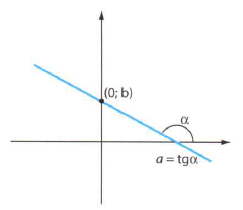
\includegraphics[width=1\linewidth]{8FMA111_imagens/imagem1}
		
	\end{multicols}
	\noindent\textsubscript{--------------------------------------------------------------------------------------------------------------------------------------------------------------}
	\begin{multicols}{2}
		\begin{enumerate} 
			\item Obtenha a equação reduzida e esboce um gráfico das seguintes equações de retas:
			\begin{enumerate}[a)]
				\item $y - x - 5 = 0$ \\\\\\\\\\\\\\\\\\\\\\\\\\\\\\
				\item $\sqrt{2}x + y - 6 = 0$ \\\\\\\\\\\\\\\\\\
				\item $4y - 3x + 1 = 0$ \\\\\\\\\\\\\\\\
			\end{enumerate}
			\item Considerando as retas das equações $ax + y - 2 = 0$ e $-ax + 3y - 10 = 0$, $a \in \mathbb{R}^*$, sendo $P$ o ponto de intersecção entre elas, classifique como \textbf{V} (verdadeiras) ou \textbf{F} (falsas) as afirmações a seguir:
			\begin{enumerate}[I.]
				\item (~~) A abscissa de $P$ depende de $a$.
				\item (~~) Existem valores de $a$ para os quais as retas não se interceptam.
				\item (~~) Se $P = (1, 3)$, uma das retas tem inclinação 45°. \\\\\\\\\\\\\\\\\\\\\\\\
			\end{enumerate}
			\item Qual a área da região do 1º quadrante delimitada pelos eixos coordenados e as retas de equação $y = -x + 3$ e $y = 3x + 2$. \\\\\\\\\\\\\\\\\\
			%1 a 4
			\item Determinar as equações gerais das retas $ \overleftrightarrow{AB}, \overleftrightarrow{AC}$ e $\overleftrightarrow{BC}$, sendo $A = (1; 0), B = (2; 3)$ e $C = (0; 5)$. \\\\\\\\\\\\\\\\\\\\\\\\\\\\\\\\
			\item Prove que as retas das equações $5x - 2y - 9 = 0, x - y = 0$ e $2x - 3y + 3 = 0$ se intersectam no mesmo ponto e determine esse ponto.  \\\\\\\\\\\\\\\\\\\\\\\\\\\\\\
			\item Determine o valor de $x$ para que os pontos $A = (1; 7), B = (-1; 3)$ e $C = (x; 15)$ pertençam a uma mesma reta. \\\\\\\\\\\\\\\\\\\\\\\\\\\\\\\\\\\\\\\\\\\\\\\\\\\\\\\\\\\\\\\\\\\\\\\\
			\item Determinar uma equação geral e a equação reduzida da reta $r$ a seguir. \\
			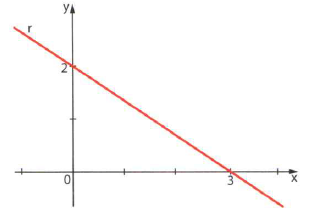
\includegraphics[width=1\linewidth]{8FMA111_imagens/imagem2}
		\end{enumerate}
		$~$ \\ 	$~$ \\ 	$~$ \\ 	$~$ \\ 	$~$ \\ 	$~$ \\ 	$~$ \\ 	$~$ \\ 	$~$ \\ 	$~$ \\ 	$~$ \\ 	$~$ \\ 	$~$ \\ 	$~$ \\ 	$~$ \\ 	$~$ \\ 	$~$ \\ 	$~$ \\ 	$~$ \\ 	$~$ \\ 	$~$ \\ 	$~$ \\ 	$~$ \\ 	$~$ \\ 	$~$ \\ 	$~$ \\ 	$~$ \\ 	$~$ \\
	\end{multicols}
\end{document}